\chapter{Warsaw WAN}

\section{Site Overview}
The Warsaw site is one of the three main locations in the \ac{RECOMP} Corporation architecture. His structure includes the following key components:
\begin{itemize}
    \item Tree core multilayer switches (3560-24PS model).
    \item One router (2901 model).
    \item Four layer 2 switches (2960-24TT model).
    \item  Four PCs representing each of the networks (STAFF, ACCOUNTING, HR, USERS).
    \end{itemize}


The topology of the warsaw site is illustrated in Figure~\ref{fig:warsaw-topology}, showcasing the interconnections between the core switches, router, layer 2 switches, and PCs.

\begin{figure}[h!]
    \centering
    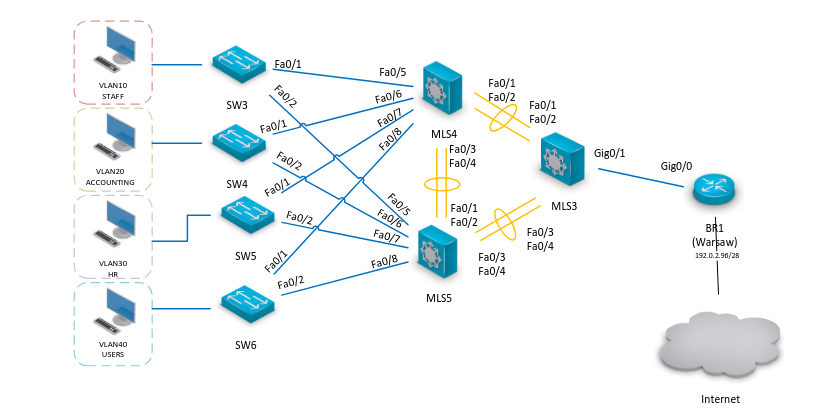
\includegraphics[width=0.9\textwidth]{figures/warsaw-topology.png}
    \caption{Warsaw Site Topology}
    \label{fig:warsaw-topology}
\end{figure}



\section{IP Addressing Scheme}
The Warsaw network architecture is built upon a structured IP plan. The following tables detail the VLAN subnets and the specific IP addresses assigned to core network devices.

\section{VLAN Subnet Allocation}

\begin{table}[h!]
\centering
\caption{VLAN Subnet Allocation}
\resizebox{\textwidth}{!}{%
\begin{tabular}{|l|c|c|c|c|c|}
\hline
\textbf{VLAN Name} & \textbf{VLAN ID} & \textbf{Network ID} & \textbf{Mask} & \textbf{Usable IP Range} & \textbf{Broadcast} \\
\hline
USERS & 40 & 192.168.162.0 & /24 & 192.168.162.1 -- 192.168.162.254 & 192.168.162.255 \\
\hline
STAFF & 10 & 192.168.163.0 & /27 & 192.168.163.1 -- 192.168.163.30 & 192.168.163.31 \\
\hline
ACCOUNTING & 20 & 192.168.163.32 & /27 & 192.168.163.33 -- 192.168.163.62 & 192.168.163.63 \\
\hline
HR & 30 & 192.168.163.64 & /27 & 192.168.163.65 -- 192.168.163.94 & 192.168.163.95 \\
\hline
\end{tabular}%
}
\label{tab:warsaw-vlan}
\end{table}

As the figure \ref{fig:warsaw-addressing} shows, the VLANs were designed to accommodate the minimum number of hosts required, also with additional capacity for future growth.

\begin{figure}[h!]
    \centering
    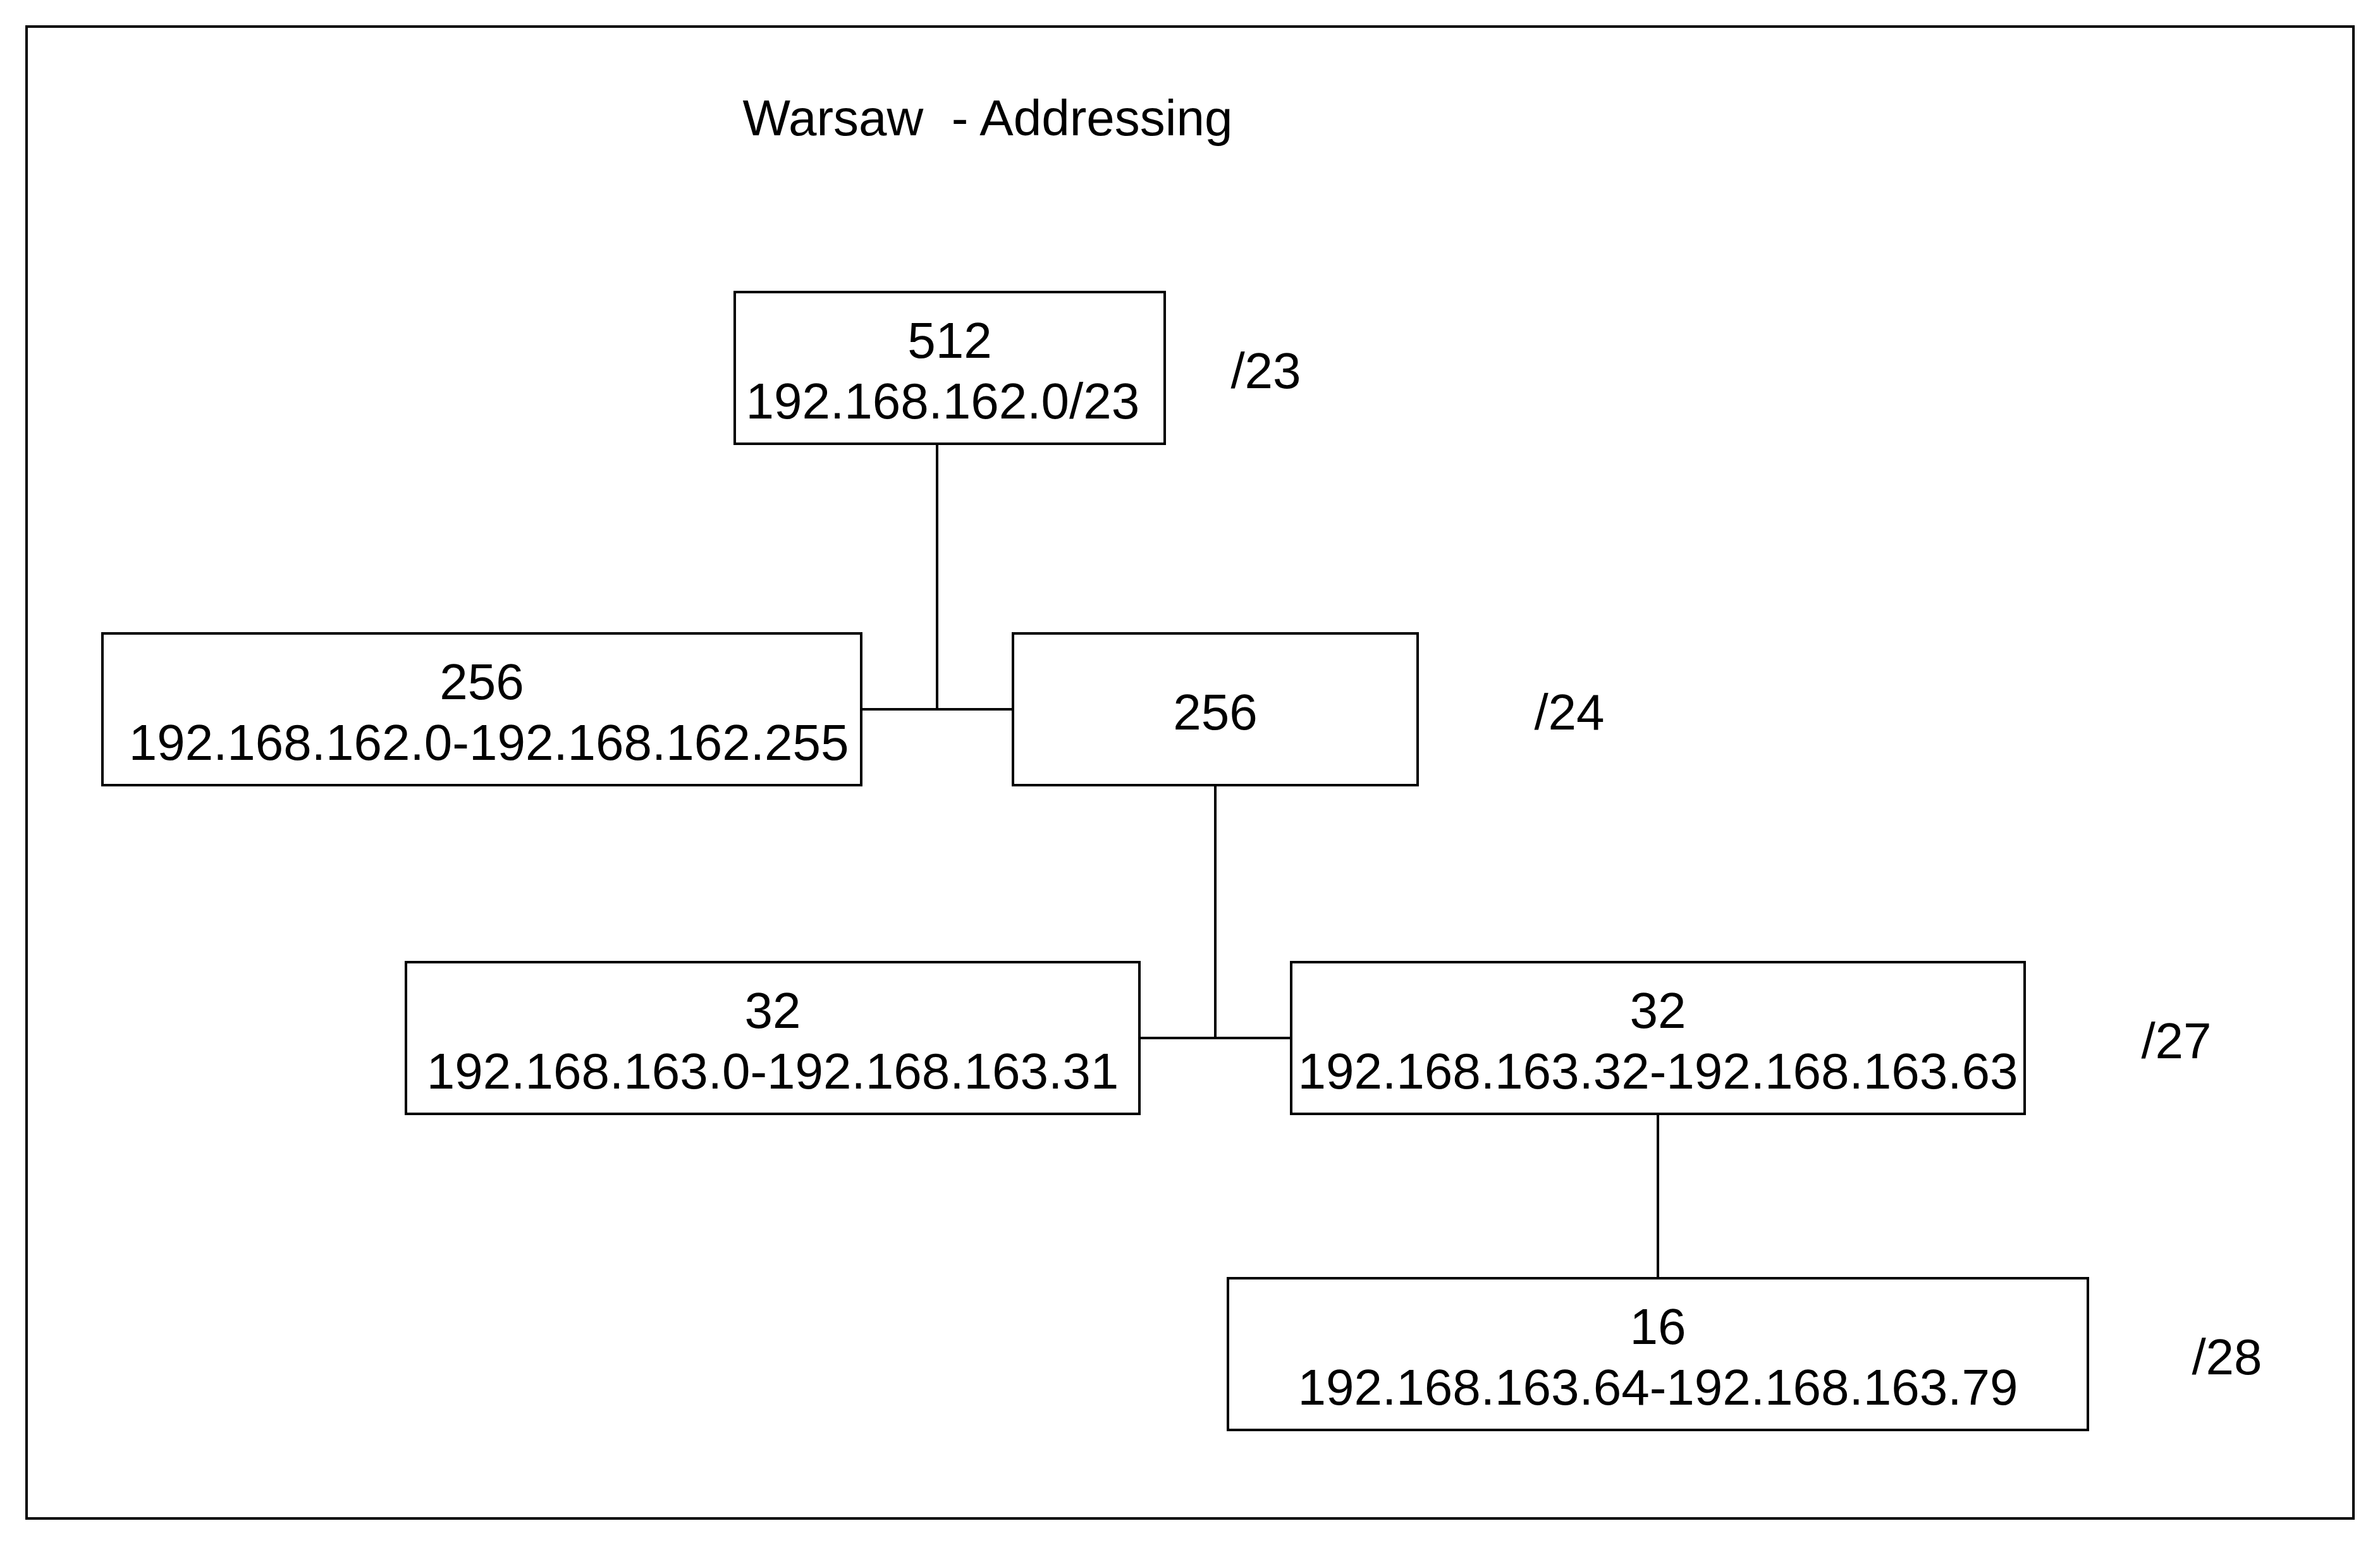
\includegraphics[width=0.9\textwidth]{figures/warsaw-addressing.png}
    \caption{Warsaw IP Addressing Scheme}
    \label{fig:warsaw-addressing}
\end{figure}    

\section{Core Device Interface Assignments}

Static IP addresses were assigned to core multilayer switch (MLS) interfaces for routing.
\begin{table}[h!]
\centering
\caption{Core Device Interface Assignments}
\begin{tabular}{|l|l|c|}
\hline
\textbf{Device} & \textbf{Interface} & \textbf{IP Address / Mask} \\

\hline
\multirow{5}{*}{MLS4} 
                      & VLAN 10 & 192.168.163.2 /27 \\
                      & VLAN 20 & 192.168.163.34 /27 \\
                      & VLAN 30 & 192.168.163.66 /27 \\
                      & VLAN 40 & 192.168.162.2 /24 \\
\hline
\multirow{5}{*}{MLS5} 
                      & VLAN 10 & 192.168.163.3 /27 \\
                      & VLAN 20 & 192.168.163.35 /27 \\
                      & VLAN 30 & 192.168.163.67 /27 \\
                      & VLAN 40 & 192.168.162.3 /24 \\
\hline
\end{tabular}
\label{tab:warsaw-core}
\end{table}


\section{Core Device Configuration}

The following command sets were applied to the core multilayer switches to establish VLANs, routing, and redundancy.

\subsection{VLAN and VTP Configuration}

VLAN Trunking Protocol (VTP) was configured to synchronize VLAN databases across the Warsaw switching domain.  
All multilayer switches operate in \texttt{server} mode to ensure database consistency and integrity.

\begin{lstlisting}[caption={VLAN and VTP configuration}, label={lst:warsaw-vtp}]
vtp mode server
vtp domain RECOMP2526M1A06
vtp password 6252pmocer

vlan 10
 name STAFF
vlan 20
 name ACCOUNTING
vlan 30
 name HR
vlan 40
 name USERS
vlan 50
 name NATIVE
vlan 99
 name BLACKHOLE
ip routing
\end{lstlisting}

\subsection{Spanning Tree Protocol \ac{STP} Configuration}

Rapid Per-VLAN Spanning Tree (Rapid-PVST) was enabled to maintain a loop-free topology and to provide load balancing between core switches.

\begin{lstlisting}[caption={RSTP configuration on MLS4}, label={lst:warsaw-rstp-mls4}]
spanning-tree mode rapid-pvst
spanning-tree vlan 10,20 root primary
spanning-tree vlan 30,40 root secondary
\end{lstlisting}

\begin{lstlisting}[caption={RSTP configuration on MLS5}, label={lst:warsaw-rstp-mls5}]
spanning-tree mode rapid-pvst
spanning-tree vlan 30,40 root primary
spanning-tree vlan 10,20 root secondary
\end{lstlisting}

\subsection{\ac{HRSP} Configuration}
HRSP was configured on both on MLS4 and MLS5 to provide gateway redundancy for endpoint devices.The following example shows the configuration for VLAN~10 (STAFF); similar configurations were applied for all other VLANs.
\begin{lstlisting}[caption={HRSP configuration for VLAN10 on MLS4/MLS5}, label={lst:warsaw-hrsp}]
    
interface vlan 10
 ip address 192.168.163.2 255.255.255.224
 standby 10 ip 192.168.163.1
 standby 10 priority 110
 standby 10 preempt
 no shutdown
exit
\end{lstlisting}



\subsection{DHCP Service Configuration}

DHCP services were configured on MLS4 and MLS5 to automate IP address assignment for endpoint devices.  
The following example shows the configuration for the VLAN~10 (STAFF) pool; similar pools were created for all other VLANs.

\begin{lstlisting}[caption={DHCP configuration for VLAN10 on MLS4/MLS5}, label={lst:warsaw-dhcp}]
ip dhcp pool VLAN10_STAFF
 network 192.168.163.0 255.255.255.224
 default-router 192.168.163.1
 dns-server 8.8.8.8
 domain-name RECOMP2526M1A06.recomp.com
exit
\end{lstlisting}
